\documentclass[11pt,letterpaper,final] {article}

%%%%%%%%%%%%%%%%%%%%%%%%%%%%%%
% Packages
%%%%%%%%%%%%%%%%%%%%%%%%%%%%%%

	\usepackage[margin=1in]{geometry}
	\usepackage{amsmath}
	\usepackage{amsfonts}
	\usepackage{fancyhdr}
	\usepackage{graphicx}
	\usepackage{apacite}
	% \usepackage{tikz}
	% \usepackage{setspace}
	% \usepackage{multicol}

%%%%%%%%%%%%%%%%%%%%%%%%%%%%%%
% Page styling
%%%%%%%%%%%%%%%%%%%%%%%%%%%%%%
	
	%%%%%%%%%%%%%%%%%%%%
	% Headers and footers
	%%%%%%%%%%%%%%%%%%%%
	
	\pagestyle{fancy}
	\renewcommand{\headrulewidth}{0pt}
	\fancyhead{}
	\fancyfoot{}
	\rhead{\thepage}
	\lhead{Wetherill}
	
	%%%%%%%%%%%%%%%%%%%%
	% Graphics path
	%%%%%%%%%%%%%%%%%%%%
	
	\graphicspath{{./}}
	
	%%%%%%%%%%%%%%%%%%%%
	% Frontmatter
	%%%%%%%%%%%%%%%%%%%%
	
	% \title{The Title}
	% \author{The Author}
	% \date{\today}

%%%%%%%%%%%%%%%%%%%%%%%%%%%%%%
% Custom definitions
%%%%%%%%%%%%%%%%%%%%%%%%%%%%%%
	% Easy scientific notation
	\newcommand{\e}[1]{\ensuremath{\times 10^{#1}}}
	
	% Textual subscripts
	\newcommand{\sub}[1]{\ensuremath{_{\text{#1}}}}
	
	% Textual superscripts
	\newcommand{\super}[1]{\ensuremath{^{\text{#1}}}}

\begin{document}
% \maketitle

\noindent Christopher Wetherill\\
TBMH 5054\\

\begin{center}
Immune Dysfunction and SLE Pathogenesis
\end{center}

Systemic lupus erythematosus (SLE) is an autoimmune disorder in which autoantibody production results in chronic inflammatory damage to multiple host organ systems \cite{Dong:2011}. Emerging evidence suggests that populations of T\sub{H} cells produce IgG class-switched autoantibodies that contribute to the pathogenesis of lupus \cite{Datta:2005}. In such a model, stylized in Figure \ref{fig:01}, we see inappropriate T\sub{H} cell activation following inappropriate recognition by B cells (or other antigen presenting cells) of autoantigens and subsequent loading of those peptide epitopes onto MHCII molecules.

\begin{figure}[htp]
  \centering
    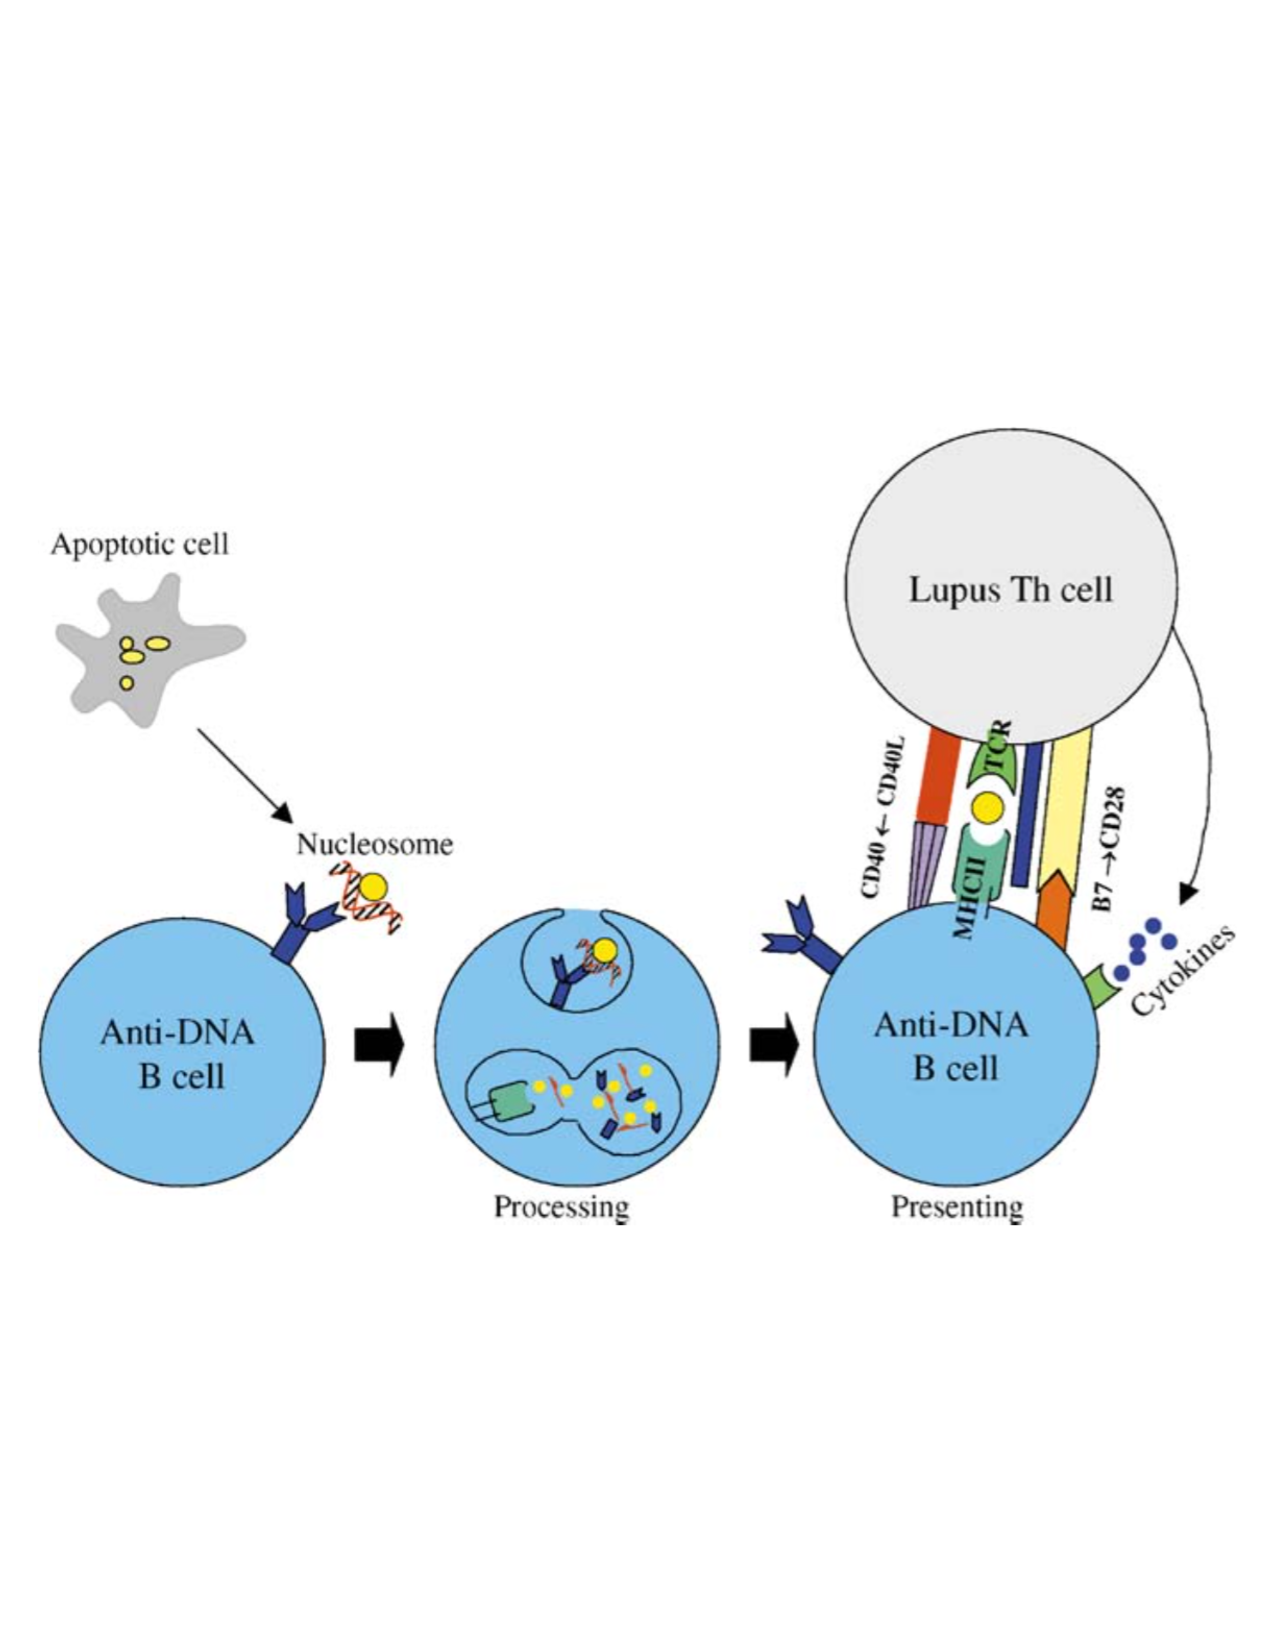
\includegraphics[width=0.65\textwidth]{sensitization}
	\caption{Stylized representation of inappropriate T\sub{H} cell activation following B cell sensitization to autoantigens. Taken from Datta, Zhang, and Xu (2005).}
	\label{fig:01}
\end{figure}

Such inappropriate activation of B cells may in part be caused by alterations to T\sub{H} cell signaling pathways. For example, it has been reported that in lupus phenotypes there is impaired cAMP-dependent phosphorylation due to reduction of protein kinase A levels; likewise, research has found compromised pathways involving protein kinase C and p56-lymphocyte-specific protein tyrosine kinase (p56lck). Further, in murine models, inhibition of the PI3K pathway and stimulation of MAPK pathways has been shown to ameliorate the disease, potentially indicating some dysfunction there acting to promote the onset of the SLE phenotype \cite{Mak:2014}.

In further studies, type I interferons have been implicated in moderating T\sub{H} cell-B cell interactions promoting autoreactivity. Specifically, triggering of plasmacytoid dendritic cell Toll-like receptors stimulates pDC secretion of IFN-$\alpha/\beta$. These interferons are, in turn, are in excess thought to promote development of autoreactive na\"{i}ve T\sub{H} cells. However, the specific role of these molecules in the development and regulation of SLE remain unclear \cite{Mangini:2007}.

Finally, recent studies have implicated T\sub{FH} cells in the pathogenesis of SLE. Specifically, the expansion of these cell populations has been found to associate with increased production of anti-dsDNA antibodies. It has been additionally hypothesized that these cell populations play a significant role in the loss of tolerance for self-reactive B cells at germinal centers: whereas self-reactive B cells would normally be excluded by germinal centers, the overabundance of T\sub{FH} cells may help to promote the survival of these B cell populations \cite{Dong:2011}. Moreover, it has been shown that inhibition of T\sub{FH} cells by inducible CD8$^{\text{+}}$ T\sub{reg} cells leads to increased self tolerance (i.e., decreased autoreactive immune response) \cite{Kim:2010}.

In summary, a wide range of immune cell dysfunctions have been implicated in SLE; however, establishing direct causative links has remained elusive. This may indicate that SLE is more accurately a spectrum of autoimmune disorders that manifest a similar phenotype but maintain separate causative agents. In any event, T\sub{H} cells seem to play a crucial role in the development and activation of autoreactive B cells and the ultimate onset of SLE and further research must be done to elucidate their exact role in the pathogenesis of this disease.

%%%%%%%%%%%%%%%%%%%%
%% REFERENCES
%%%%%%%%%%%%%%%%%%%%

\clearpage
\bibliographystyle{apacite}
\bibliography{references}
\nocite{*}

\end{document}